\documentclass[12pt]{beamer}
\usepackage{../Estilos/BeamerMAF}
\usefonttheme{serif}
\usetheme{Madrid}
\usecolortheme{whale}
%\useoutertheme{default}
\setbeamercovered{invisible}
% or whatever (possibly just delete it)
\setbeamertemplate{section in toc}[sections numbered]
\setbeamertemplate{subsection in toc}[subsections numbered]
\setbeamertemplate{subsection in toc}{\leavevmode\leftskip=3.2em\rlap{\hskip-2em\inserttocsectionnumber.\inserttocsubsectionnumber}\inserttocsubsection\par}
% \setbeamercolor{section in toc}{fg=blue}
% \setbeamercolor{subsection in toc}{fg=blue}
% \setbeamercolor{frametitle}{fg=blue}
\setbeamertemplate{caption}[numbered]

\setbeamertemplate{footline}
\beamertemplatenavigationsymbolsempty
\setbeamertemplate{headline}{}


\makeatletter
% \setbeamercolor{section in foot}{bg=gray!30, fg=black!90!orange}
% \setbeamercolor{subsection in foot}{bg=blue!30}
% \setbeamercolor{date in foot}{bg=black}
\setbeamertemplate{footline}
{
  \leavevmode%
  \hbox{%
  \begin{beamercolorbox}[wd=.333333\paperwidth,ht=2.25ex,dp=1ex,center]{section in foot}%
    \usebeamerfont{section in foot} \insertsection
  \end{beamercolorbox}%
  \begin{beamercolorbox}[wd=.333333\paperwidth,ht=2.25ex,dp=1ex,center]{subsection in foot}%
    \usebeamerfont{subsection in foot}  \insertsubsection
  \end{beamercolorbox}%
  \begin{beamercolorbox}[wd=.333333\paperwidth,ht=2.25ex,dp=1ex,right]{date in head/foot}%
    \usebeamerfont{date in head/foot} \insertshortdate{} \hspace*{2em}
    \insertframenumber{} / \inserttotalframenumber \hspace*{2ex} 
  \end{beamercolorbox}}%
  \vskip0pt%
}
\makeatother

\makeatletter
\patchcmd{\beamer@sectionintoc}{\vskip1.5em}{\vskip0.8em}{}{}
\makeatother


%Reduce el espacio entre los items de la TOC
\makeatletter
\patchcmd{\beamer@sectionintoc}{\vskip1.5em}{\vskip0.8em}{}{}
\setbeamercolor{section in foot}{bg=ballblue, fg=white}
\setbeamercolor{subsection in foot}{bg=ao, fg=white}
\setbeamercolor{date in foot}{bg=black, fg=white}

\makeatother

\title{Matemáticas Avanzadas de la Física}
\subtitle{Semestre 2022-2}

\newcommand\RBox[1]{%
  \tikz\node[draw,rounded corners,align=center,] {#1};%
}

\date{11 de febrero de 2022}

\begin{document}
\maketitle

\begin{frame}
\frametitle{Equipo académico}
\begin{center}
\RBox{
M. en C. Gustavo Contreras Mayén \\
\href{mailto:gux7avo@ciencias.unam.mx}{gux7avo@ciencias.unam.mx}
}
\vskip 1cm
\RBox{
M. en C. Abraham Lima Buendía \\
\href{mailto:abraham3081@ciencias.unam.mx}{abraham3081@ciencias.unam.mx}
}
\end{center}
\end{frame}

\section*{Contenido}
\frame{\frametitle{Contenido}\tableofcontents[currentsection, hideallsubsections]}
\fontsize{14}{14}\selectfont
\spanishdecimal{.}

\section{Presentación del curso}
\frame{\frametitle{Contenido}\tableofcontents[currentsection, hideothersubsections]}
\subsection{Objetivos}

\begin{frame}
\frametitle{Objetivos del curso}
En la página de la Facultad, el programa de la asignatura: Matemáticas Avanzadas de la Física se puede consultar \href{http://www.fciencias.unam.mx/asignaturas/610.pdf}{(aquí)}, y contiene los siguientes objetivos:
\end{frame}
\begin{frame}
\frametitle{Objetivos del curso}
En donde el alumno:
\begin{itemize}[<+->]
\setlength{\itemsep}{0mm}
\item Reconocerá las ideas básicas del análisis de ecuaciones que involucran a funciones de varias variables.
\item Formulará aproximaciones consistentes a soluciones, con el fin de cuantificar los distintos mecanismos de la física que se involucran.
\end{itemize}
\end{frame}
\begin{frame}
\frametitle{Objetivos del curso}
Además:
\begin{itemize}[<+->]
\setlength{\itemsep}{0mm}
\item Consultará la literatura matemática que sea relevante para los problemas de física.
\item Identificará el papel moderno que juegan las funciones especiales, como auxiliares poderosos en el análisis cualitativo de problemas en varias variables.
\end{itemize}
\end{frame}
\begin{frame}
\frametitle{Objetivo adicional}
También es nuestro objetivo demostrar al alumno que \emph{las funciones especiales y las transformadas integrales} no son solamente un tema matemático, que involucra las ramas de la geometría diferencial, las ecuaciones diferenciales y el análisis matemático.
\end{frame}
\begin{frame}
\frametitle{Objetivo adicional}
Veremos que \emph{son las técnicas de estudio fundamentales} en la electrostática, la electrodinámica, la mecánica cuántica en los límites relativista y no relativista, la dinámica de medios deformables, la hidrodinámica clásica entre otras ramas de la física.
\end{frame}
\begin{frame}
\frametitle{Relevancia de la asignatura}
MAF les brindará un manejo más fluido y consistente para lo que van a cursar en el sexto semestre y los tres semestres que les restan para concluir la carrera.
\\
\bigskip
\pause
Es una asignatura con bastante relevancia para la formación del físico.
\end{frame}

\section{Metodología de enseñanza}
\frame[allowframebreaks]{\tableofcontents[currentsection, hideothersubsections]}
\subsection{Semestre a distancia/presencial}

\begin{frame}
\frametitle{Situación para el inicio del semestre}
De acuerdo con el mensaje enviado por las autoridades de la Facultad de Ciencias, el semestre 2022-2 tendrá una modalidad de trabajo a distancia \emph{durante las primeras cuatro semanas}.
\end{frame}
\begin{frame}
\frametitle{Asignación de modalidad}
Se espera que el Consejo Técnico determine cuáles asignaturas se impartirán en modalidad presencial y cuáles continuarán en modalidad a distancia.
\end{frame}
\begin{frame}
\frametitle{Modalidad presencial}
En caso de que el Consejo Técnico determine que la asignatura se imparta en modalidad presencial, se continuará el trabajo de acuerdo al programa de trabajo en los días establecidos: \textbf{martes} y \textbf{jueves}  a las 3 pm en el aula que se indique.
\end{frame}
\begin{frame}
\frametitle{Modalidad a distancia}
En caso de que se nos indique que el curso se imparta en modalidad a distancia, continuaremos con el esquema de trabajo planteado, así como con las videoconferencias en los días y horarios de clase. 
\end{frame}

{
\setbeamercolor{background canvas}{bg=}
\includepdf[pages=1]{Calendario_Esquema_Trabajo_2022_2_01.pdf}
}

{
\setbeamercolor{background canvas}{bg=}
\includepdf[pages=1]{Calendario_Esquema_Trabajo_2022_2_02.pdf}
}

\begin{frame}
\frametitle{Plataforma de trabajo}
Para este curso tanto para las primeras cuatro semanas y en caso de que todo el semestre sea a distancia,  utilizaremos la plataforma Moodle, favoreciendo una estandarización con las demás asignaturas que se imparten en la Facultad de Ciencias.
\end{frame}
\begin{frame}
\frametitle{Plataforma Moodle}
\begin{figure}
\centering

\includegraphics[scale=0.2]{Imagenes/Moodle_Ciencias.png}
\end{figure}
\end{frame}
\begin{frame}
\frametitle{Acceso a Moodle}
Se proporcionarán las credenciales para ingresar a la plataforma en donde encontrarán las actividades de trabajo, materiales de consulta y referencias adicionales para el curso.
\end{frame}
\begin{frame}
\frametitle{Materiales de trabajo}
Se contará con materiales que deberán de revisar: en ellos se discute el tema, dentro de los materiales se incluyen ejemplos.
\\
\bigskip
La lectura y trabajo con estos materiales es \emph{obligatoria.}
\end{frame}
\begin{frame}
\frametitle{Materiales adicionales}
De manera complementaria se dispondrá de materiales adicionales de consulta, en ellos se hará un revisión en particular de un ejercicio o problema.
\end{frame}
\begin{frame}
\frametitle{Materiales adicionales}
Buscando que el desarrollo se aborde con otro enfoque, pero que complementa lo que hayan revisado en los materiales de trabajo.
\\
\bigskip
Recomendamos mucho que revisen estos materiales adicionales.
\end{frame}
\begin{frame}
\frametitle{Canal de YouTube}
Se han elaborado videos en donde se trabajan ejercicios y ejemplos para los temas.
\\
\bigskip
\pause
Dentro de Moodle se estarán incorporando las ligas para el canal de Youtube, de tal manera que podrán revisar los videos en el momento que ustedes consideren oportuno.
\end{frame}
\begin{frame}
\frametitle{Canal en YouTube}
\begin{figure}[H]
  \centering
  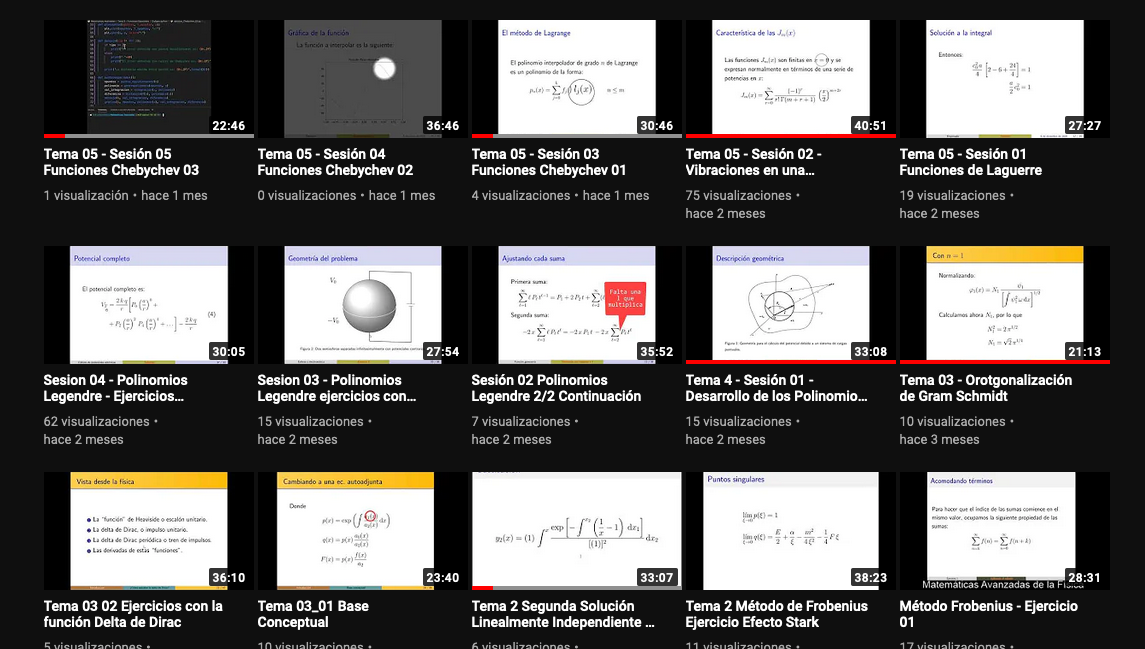
\includegraphics[scale=0.25]{Imagenes/canal_videos.png}
\end{figure}
\end{frame}

\subsection{Tiempo para atender el curso}

\begin{frame}
\frametitle{Requerimiento de tiempo}
De manera independiente a la modalidad de trabajo, deben de considerar \enquote{apartar} tiempo para la asignatura, por lo que hacemos la recomendación de que midan su carga académica durante este semestre.
\end{frame}
\begin{frame}
\frametitle{Comunicación constante}
Además de contar con los correos electrónicos, se estará utilizando un canal de Telegram para el envío de mensajes generales, así como para notificaciones, avisos, etc.
\\
\bigskip
\begin{figure}
    \centering
    
\includegraphics[scale=0.15]{Imagenes/Logo_Telegram.png}
\end{figure}
\end{frame}
\begin{frame}
\frametitle{Liga y clave para la videoconferencia}
El envío de la liga y las claves de ingreso a las sesiones de Zoom, se hará por correo, nunca por Telegram.
\\
\bigskip
De esta manera se evita que haya ingresos indebidos a las reuniones.
\end{frame}
\begin{frame}
\frametitle{Material de consulta}
Se contará con diversos materiales de consulta: artículos, capítulos de libros, etc. que estarán disponibles tanto en la plataforma Moodle como en la nube de Drive, por lo que tendrán oportunidad de consultarlos libremente.
\end{frame}

\section{Evaluación}
\frame[allowframebreaks]{\small\tableofcontents[currentsection, hideothersubsections]}
\subsection{Elementos para la calificación.}

\begin{frame}
\frametitle{Elementos para la calificación}
El porcentaje para cada elemento de evaluación es el siguiente:
\begin{itemize}
\setlength{\itemsep}{0mm}
\item Exámenes - Tarea: $\mathbf{80\%}$.
\item Ejercicios: $\mathbf{20\%}$.
\end{itemize}
\end{frame}

\subsection{Ejercicios por tema}

\begin{frame}
\frametitle{Ejercicios por tema}
Por cada tema del curso, se incluyen 10 ejercicios a resolver. El listado de ejercicios se entregará cuando inicie el tema, para que de esta manera, se vayan resolviendo, a la vez de contar con la oportunidad para hacer consultas, orientaciones, etc.
\\
\bigskip
\pause
Al concluir el tema, se deberá de enviar la solución por Moodle a la siguiente semana.
\end{frame}
\begin{frame}
\frametitle{Muy importante}
Cada ejercicio aporta un punto, siempre y cuando esté bien resuelto.
\\
\bigskip
\pause
En caso de que que el ejercicio no se haya resuelto debidamente, se otorgará una parte proporcional del punto. \pause Recomendamos ampliamente la solución de todos los ejercicios.
\end{frame}
\begin{frame}
\frametitle{Ejercicios resueltos - Puntaje}
En la siguiente tabla se indica el puntaje obtenido a partir de los ejercicios resueltos y enviados.
\\
\bigskip
\pause
El puntaje que se otorga considera que cada ejercicio se resolvió debidamente y obtuvo $1$ punto.
\end{frame}
\begin{frame}
\frametitle{Ejercicios resueltos - Puntaje}
\begin{table}
\centering
\renewcommand{\arraystretch}{1.1}
\begin{tabular}{c | c}
Ejercicios & Puntos \\ \hline
$10$ & $0.333$  \\ \hline
$20$ & $0.666$ \\ \hline
$30$ & $1$ \\ \hline
$40$ & $1.333$ \\ \hline
$50$ & $1.666$ \\ \hline
$60$ & $2$ \\ \hline
\end{tabular}
\end{table}
\end{frame}
\begin{frame}
\frametitle{Muy importante 2}
Se deben de enviar y/o entregar los ejercicios en la fecha señalada.
\\
\bigskip
\pause
No se reciben envíos extemporáneos.
\end{frame}

\subsection{Exámenes - Tarea}

\begin{frame}
\frametitle{Exámenes - Tarea}
Habrá dos exámenes durante el curso.
\\
\bigskip
\pause
\setbeamercolor{item projected}{bg=blue!70!black,fg=yellow}
\setbeamertemplate{enumerate items}[circle]
\begin{enumerate}[<+->]
\item Un examen intermedio (Temas 1, 2, 3)
\item Un examen al final (Temas 4, 5, 6)
\end{enumerate}
\end{frame}
\begin{frame}
\frametitle{Exámenes - Tarea}
Se entregarán los enunciados de cada examen al inicio del tema, de esta manera se tendrá el suficiente tiempo para la solución y entrega del mismo.
\\
\bigskip
\pause
En promedio se incluirán 6 preguntas por cada tema.
\end{frame}
\begin{frame}
\frametitle{Exámenes - Tarea}
El Examen - Tarea se debe de entregar completo, en caso de que no suceda así, se tomará la respectiva parte proporcional de la calificación obtenida.
\end{frame}
\begin{frame}
\frametitle{De los Exámenes y Ejercicios}
Durante la evaluación de los ejercicios de los exámenes y ejercicios  \emph{se revisa y se evalúa el proceso de resolución de un problema, es decir, será necesario detallar cada paso en la solución}.
\\
\bigskip
\pause
Los ejercicios por Tema así como los exámenes tendrán que ser resueltos a mano.
\end{frame}
\begin{frame}
\frametitle{Punto importante}
En la solución se deberá de detallar cada paso que se realice.
\\
\bigskip
\pause
No se recibirán soluciones que indiquen comprobaciones hechas en \emph{Mathematica, MatLab, Maple, etc.}
\end{frame}
\begin{frame}
\frametitle{¿Cómo entregar los Ejercicios y Exámenes?}
\textbf{Modalidad presencial y a distancia. } Si cuentan con un escáner, se deberá de digitalizar cada una de las hojas que hayan ocupado en un archivo pdf y enviarlo mediante la plataforma.
\\
\bigskip
\pause
En caso de no contar con un escáner para la digitalización de las soluciones, se podrá enviar un archivo con las imágenes de la solución, tomadas con una tableta o el celular.
\end{frame}
\begin{frame}
\frametitle{De los Ejercicios y Exámenes}
Se les pedirá encarecidamente, ser lo más claros en la escritura, numeración de las hojas, el orden y limpieza en sus soluciones, para que así recibamos un archivo que nos permita evaluar su trabajo.
\end{frame}

\subsection{Consideraciones importantes}

\begin{frame}
\frametitle{Consideraciones importantes}
\begin{itemize}
\setlength{\itemsep}{0mm}
\item No se recibirán Ejercicios de manera extemporánea, en Moodle quedarán programada la fecha y horario para el envío, una vez que se llega al tiempo indicado, la plataforma ya no permite el envío.
\item No habrá reposición de exámenes.
\end{itemize}
\end{frame}
\begin{frame}
\frametitle{Consideraciones importantes}
\begin{itemize}
\setlength{\itemsep}{0mm}
\item En caso de que la calificación de un Examen - Tarea (o los dos) sea menor a $6$ (seis), el alumno presentará el Examen Final de todo el curso.
\item Para presentar Examen Final de todo el curso se requiere que el alumno haya entregado los dos Exámenes -  Tarea del curso.
\end{itemize}
\end{frame}
\begin{frame}
\frametitle{Consideraciones importantes}
\begin{itemize}
\setlength{\itemsep}{0mm}
\item En caso de no haber entregado ningún bloque de Ejercicios y no haber presentado los dos Exámenes del curso, no se tendrá derecho a presentar el Examen Final, por lo que la calificación final que se asentará en el acta del curso, será \textbf{NP (No presentó)}.
\end{itemize}
\end{frame}
\begin{frame}
\frametitle{Consideraciones importantes}
\begin{itemize}
\setlength{\itemsep}{0mm}
\item En caso de haber presentado al menos un Examen - Tarea y/o haber entregado un bloque de Ejercicios, y posteriormente no se tenga registro de otra entrega, se entenderá que abandonaron el curso, por lo que no se tendrá derecho para presentar el Examen Final, y la calificación que se asentará en el acta del curso, será $\mathbf{5}$ \textbf{(cinco)}.
\end{itemize}
\end{frame}
\begin{frame}
\frametitle{Ejemplo de evaluaciones}
\fontsize{12}{12}\selectfont
\begin{table}
\begin{tabular}{| l | c | c | c | c | c | c | c | c |} \hline
& \multicolumn{5}{c |}{Ejercicios} & \multicolumn{2}{c |}{Exámenes} & \\ \hline
Alumno & T1 & T2 & $\ldots$ & T5 & T6 & E1 & E2 & Final \\ \hline
C. López & $9.0$ & $6.3$ & $\ldots$ & $0$ & $0$ & $8.3$ & $0 $ & $\mathbf{5}$ \\ \hline \pause 
J. Nieves & $0$ & $0$ & $\ldots$ & $0$ & $0$ & $0$ & $0$ & \textbf{NP} \\ \hline
\end{tabular}
\end{table}
\end{frame}
\begin{frame}
\frametitle{Consideraciones importantes}
\begin{itemize}[<+->]
\setlength{\itemsep}{0mm}
\item En caso de presentar la primera ronda del Examen Final y la calificación obtenida sea no aprobatoria ($<6.0$), se puede presentar una segunda y última ronda del Examen Final.
\item La calificación obtenida en el Examen Final, es la que se asentará en actas.
\item Si el alumno no presenta el primer Examen Final, tendrá como calificación final en acta $\mathbf{5}$ \textbf{(cinco)}. 
\end{itemize}
\end{frame}

\section{Temario}
\frame[allowframebreaks]{\small\tableofcontents[currentsection, hideothersubsections]}


\subsection{La física y la geometría}

\begin{frame}
\frametitle{Tema 1 - La física y la geometría}
\setbeamercolor{item projected}{bg=blue!70!black,fg=yellow}
\setbeamertemplate{enumerate items}[circle]
\begin{enumerate}[<+->]
\item Sistemas de coordenadas curvilíneas ortogonales.
\item Operadores diferenciales en coordenadas curvilíneas.
\item Funciones Gamma y Beta.
\end{enumerate}
\end{frame}

\subsection{Primeras técnicas de solución}

\begin{frame}
\frametitle{Tema 2 - Primeras técnicas de solución}
\setbeamercolor{item projected}{bg=blue!70!black,fg=yellow}
\setbeamertemplate{enumerate items}[circle]
\begin{enumerate}[<+->]
\item Técnica de separación de variables.
\item Método de Frobenius y remoción de singularidades.
\item Segunda solución linealmente independiente.
\item Función de Green.
\end{enumerate}
\end{frame}

\subsection{Bases completas y ortogonales}

\begin{frame}
\frametitle{Tema 3 - Bases completas y ortogonales}
\setbeamercolor{item projected}{bg=blue!70!black,fg=yellow}
\setbeamertemplate{enumerate items}[circle]
\begin{enumerate}[<+->]
\item La delta de Dirac. 
\item Ecuaciones de tipo Sturm-Liouville.
\item Ortogonalización de Gram-Schimdt.
\item Completes de las funciones propias.
\end{enumerate}
\end{frame}

\subsection{Sep. variables en coord. esféricas}
\begin{frame}
\frametitle{Tema 4 - Sep. de variables en coord. esféricas}
\framesubtitle{Análisis del átomo de hidrógeno}
\setbeamercolor{item projected}{bg=blue!70!black,fg=yellow}
\setbeamertemplate{enumerate items}[circle]
\begin{enumerate}[<+->]
\item \textcolor{blue}{Parte radial}: Ec. asociada de Laguerre. y la Ec. ordinaria de Laguerre.
\item \textcolor{blue}{Parte angular}:
\item Armónicos esféricos.
\item Teorema de adición.
\item Ecuación asociada de Legendre y la Ecuación ordinaria de Legendre.
\end{enumerate}
\end{frame}

\subsection{Funciones especiales}

\begin{frame}
\frametitle{Tema 5 - Funciones especiales}
\setbeamercolor{item projected}{bg=blue!70!black,fg=yellow}
\setbeamertemplate{enumerate items}[circle]
\begin{enumerate}[<+->]
\item Funciones de Bessel. (Propagación de ondas cilíndricas)
\item Funciones de Hermite. (Oscilador armónico cuántico)
\item Funciones de Chebychev (Interpolación numérica)
\item Funciones hipergeométricas: ordinaria y confluente.
\item Funciones de Gegenbauer.
\end{enumerate}
\end{frame}
\subsection{Transformadas integrales}
\begin{frame}
\frametitle{Tema 6 - Transformadas integrales}
\setbeamercolor{item projected}{bg=blue!70!black,fg=yellow}
\setbeamertemplate{enumerate items}[circle]
\begin{enumerate}[<+->]
\item Transformada de Fourier.
\item Transformada de Laplace.
\item Transformada discreta de Fourier.
\item Transformada rápida de Fourier.
\end{enumerate}
\end{frame}

\section{Cronograma de trabajo}
\frame{\tableofcontents[currentsection, hideothersubsections]}
\subsection{Calendarización del curso}

\begin{frame}
\frametitle{Calendarización}
A continuación se presenta el cronograma de trabajo para el curso, durante las 16 semanas del semestre se han distribuido los 6 temas.
\end{frame}
{
\setbeamercolor{background canvas}{bg=}
\includepdf[pages=1-5]{Calendario_2022_2.pdf}
}

\section{Fechas importantes}
\frame{\tableofcontents[currentsection, hideothersubsections]}
\subsection{Calendario oficial}

\begin{frame}
\frametitle{Fechas importantes}
%\fontsize{12}{12}\selectfont
\begin{itemize}[<+->]
\item \textcolor{red}{Lunes 14 de febrero de 2022. Inicio del semestre 2022-2.}
\item \textcolor{blue}{Del Lunes 11 al viernes 15 de abril de 2022. Período Vacacional de Semana Santa.}
\item Martes 10 de mayo de 2022. Día feriado.
\item \textcolor{red}{Viernes 10 de junio. Termina el semestre 2022-2.}
\end{itemize}
\end{frame}
\begin{frame}
\frametitle{Fechas importantes - Por confirmar}
%\fontsize{12}{12}\selectfont
\begin{itemize}[<+->]
\item Del lunes 13 al viernes 17 de junio de 2022. \underline{Primera semana de exámenes}.
\item Del lunes 20 al 24 de junio del 2022. \underline{Segunda semana de exámenes}.
\end{itemize}
\end{frame}
\end{document}